\documentclass[10pt,twocolumn,letterpaper]{article}

\usepackage{cvpr}
\usepackage{times}
\usepackage{epsfig}
\usepackage{graphicx}
\usepackage{amsmath}
\usepackage{amssymb}

% Include other packages here, before hyperref.

% If you comment hyperref and then uncomment it, you should delete
% egpaper.aux before re-running latex.  (Or just hit 'q' on the first latex
% run, let it finish, and you should be clear).
\usepackage[breaklinks=true,bookmarks=false]{hyperref}

\cvprfinalcopy % *** Uncomment this line for the final submission

\def\cvprPaperID{****} % *** Enter the CVPR Paper ID here
\def\httilde{\mbox{\tt\raisebox{-.5ex}{\symbol{126}}}}

% Pages are numbered in submission mode, and unnumbered in camera-ready
%\ifcvprfinal\pagestyle{empty}\fi
\setcounter{page}{4321}
\begin{document}

%%%%%%%%% TITLE
\title{\LaTeX\ Author Guidelines for CVPR Proceedings}

\author{First Author\\
Institution1\\
Institution1 address\\
{\tt\small firstauthor@i1.org}
% For a paper whose authors are all at the same institution,
% omit the following lines up until the closing ``}''.
% Additional authors and addresses can be added with ``\and'',
% just like the second author.
% To save space, use either the email address or home page, not both
\and
Second Author\\
Institution2\\
First line of institution2 address\\
{\tt\small secondauthor@i2.org}
}

\maketitle
%\thispagestyle{empty}

%%%%%%%%% ABSTRACT
\begin{abstract}
   The ABSTRACT is to be in fully-justified italicized text, at the top
   of the left-hand column, below the author and affiliation
   information. Use the word ``Abstract'' as the title, in 12-point
   Times, boldface type, centered relative to the column, initially
   capitalized. The abstract is to be in 10-point, single-spaced type.
   Leave two blank lines after the Abstract, then begin the main text.
   Look at previous CVPR abstracts to get a feel for style and length.
\end{abstract}

%%%%%%%%% BODY TEXT
\section{Introduction}

\section{Related Work}

\subsection{R-CNN}
~\cite{RCNN} addressed the R-CNN detector which promote the accuracy of nueral networks for object detection. This R-CNN detector combines a region proposal part (Selective Search~\cite{SelectiveSearch}), a CNN feature extractor and a classifer. R-CNN detector surmount conventional detectors in the aspect of accuracy but its speed is limited by generating massive region proposals and extracting features using CNN on each of the region proposal. 

Spatial pyramid pooling (SPP)~\cite{SPP} introduced a way to meliorate by employ pyramid pooling layer. SPP-net speed up the detector by computing CNN only once per image. Imitating SPP-net, Fast-RCNN ~\cite{fastRCNN} shown that using multi-task learning and back-propagation through ROI pooling layer will speed up the R-CNN detector by an order of magnitude. 

The bottleneck of Fast-RCNN is conventional region proposal generator, so Faster-RCNN ~\cite{fasterRCNN} proposed Region Proposal Network (RPN) which sharing features with classifer network.


\subsection{Region Proposal}
Most traditional region proposal methods are based on low-level features. Faster-RCNN introduced Region Proposal Network (RPN) to generate region proposals based on high-level semantic features. RPN surpass conventional region proposal methods, either unsupervised method (e.g. Selective Search~\cite{SelectiveSearch}) or supervised method (e.g. BING~\cite{BING}), on both speed and accuracy.

There are several approach of refining region proposals.

\subsubsection{cascade refinement}
Region Proposal Network can be refined by applying a multi-stage cascading pipeline structure.

CRAFT~\cite{CRAFT} uses a two-class Fast R-CNN to refine proposals generate by a standard RPN, and ~\cite{CraftingGBD} improved CRAFT. DeepBox~\cite{DeepBox} rerank proposals produced by EdgeBoxes ~\cite{EdgeBoxes} to refine proposals. DeepProposal~\cite{DeepProposal} introduce a Cascading Deep Convolutional Layers to get feature maps. Similar to CRAFT, ~\cite{Cascadedcnn} proposes a RefineNet added after RPN which can effectively reduce the number of proposals and improve their confidence. MTCNN~\cite{MTCNN} apply similar approach, using a R-net to refine P-net.

~\cite{GroupRecursive} introduce a spatial correlation related method, using a new EM-like group recursive learing approach to iteratively refine object proposals and provide an optimal spatial configuration of object detections.
\subsubsection{multi-scale refinment}
Methods like SDP,SSH or MS-CNN ~\cite{SDP}~\cite{SSH}~\cite{MSCNN}make independent prodictions at different layers, which will ensure smaller objects are trained on higher resolution layers.


Other methods like FPN, RetinaNet~\cite{FPN}~\cite{RetinaNet} propose a pyramidal structure to combine shallow layer with deep layer to get both high-level feature and low-level feature.

\subsection{ROI and NMS}
CoupleNet~\cite{CoupleNet} propose a two branch network of ROI after RPN to obtain both local part information and global imformation.



\section{Aspect Ratio Sensitive Object Detection}
\subsection{Aspect Ratio Sensitive Network}
% Insert an image of the different aspect ratio
We have count the sapect ratio of different classes on different dataset. All datasets contain certain classes whose aspect ratio show obvious uneven distribution among different shapes. 
% For example, in MSCOCO 2017, the majority of the ball is of the shape 1*1, only a few sample gets to 1*2 and 2*1.


\subsection{Network Architure}
\paragraph{ARS Net}
To include aspect ratio as a prior knowledge for object detection, we modified the network architure by duplicating the region proposal network into 3 copies, each handling objects of different shapes. During training (see figure \ref{ARS_De}), green rpn (right) is only provided with ground truth bounding boxes of aspect ratio greater than 2:1, grey one (middle) with boxes around 1:1 only and yellow one (left) with boxes smaller than 1:2 only. Results of three region proposal networks are simply stacked together in testing time. In this way, our network is able to learn separate filters for objects of different shapes. Non-maximum suppression is applied in the end to reject high over-lapping objects. 
    \begin{figure}[!htb]
    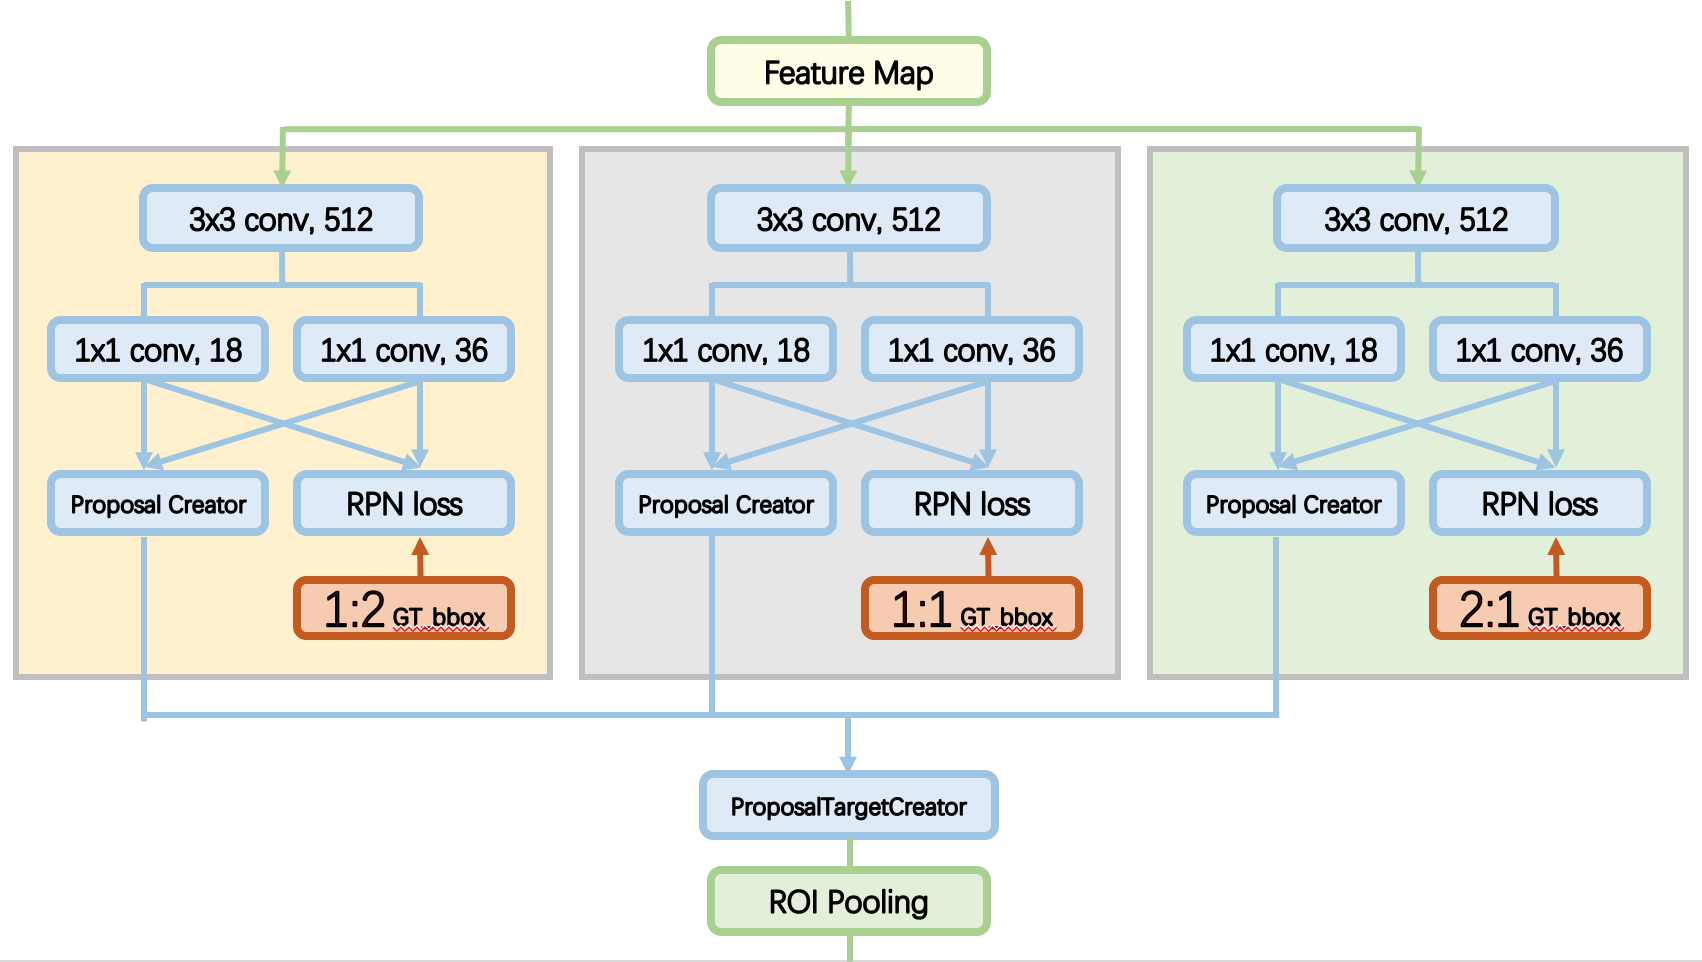
\includegraphics[width= 0.45\textwidth]{pic/ARS-archi-detail.png}
    \caption{Multiple RPN approach}
    \label{ARS_De}
    \end{figure}


\paragraph{Sharing Features}
The multi-rpn network works, but comes at great cost. One of the obvious shortcomings of this approach would be the high overall time complexity. Compared with the original faster RCNN, which runs at about 9fps on one Nvidia TitanX, our multi-rpn approach can only run at half speed. Sharing features, plus adding additional one-by-one convolutional layers are applied to cope with such problem. More specifically (see Figure \ref{ARS_sh}), three rpns share the same 3*3*512 layer, but each would have another 1*1*256 layer of its own to further reduce depth. Other parts of the network remains unchangde. From table \ref{table_fps}, adding 1*1 conv into our network improves speed while maintaining a similar mAp. However, it's still slow when compared with the origin RCNN, afterall, region proposal network still remains to be the biggest overhead of faster RCNN.
    \begin{figure}[!htb]
    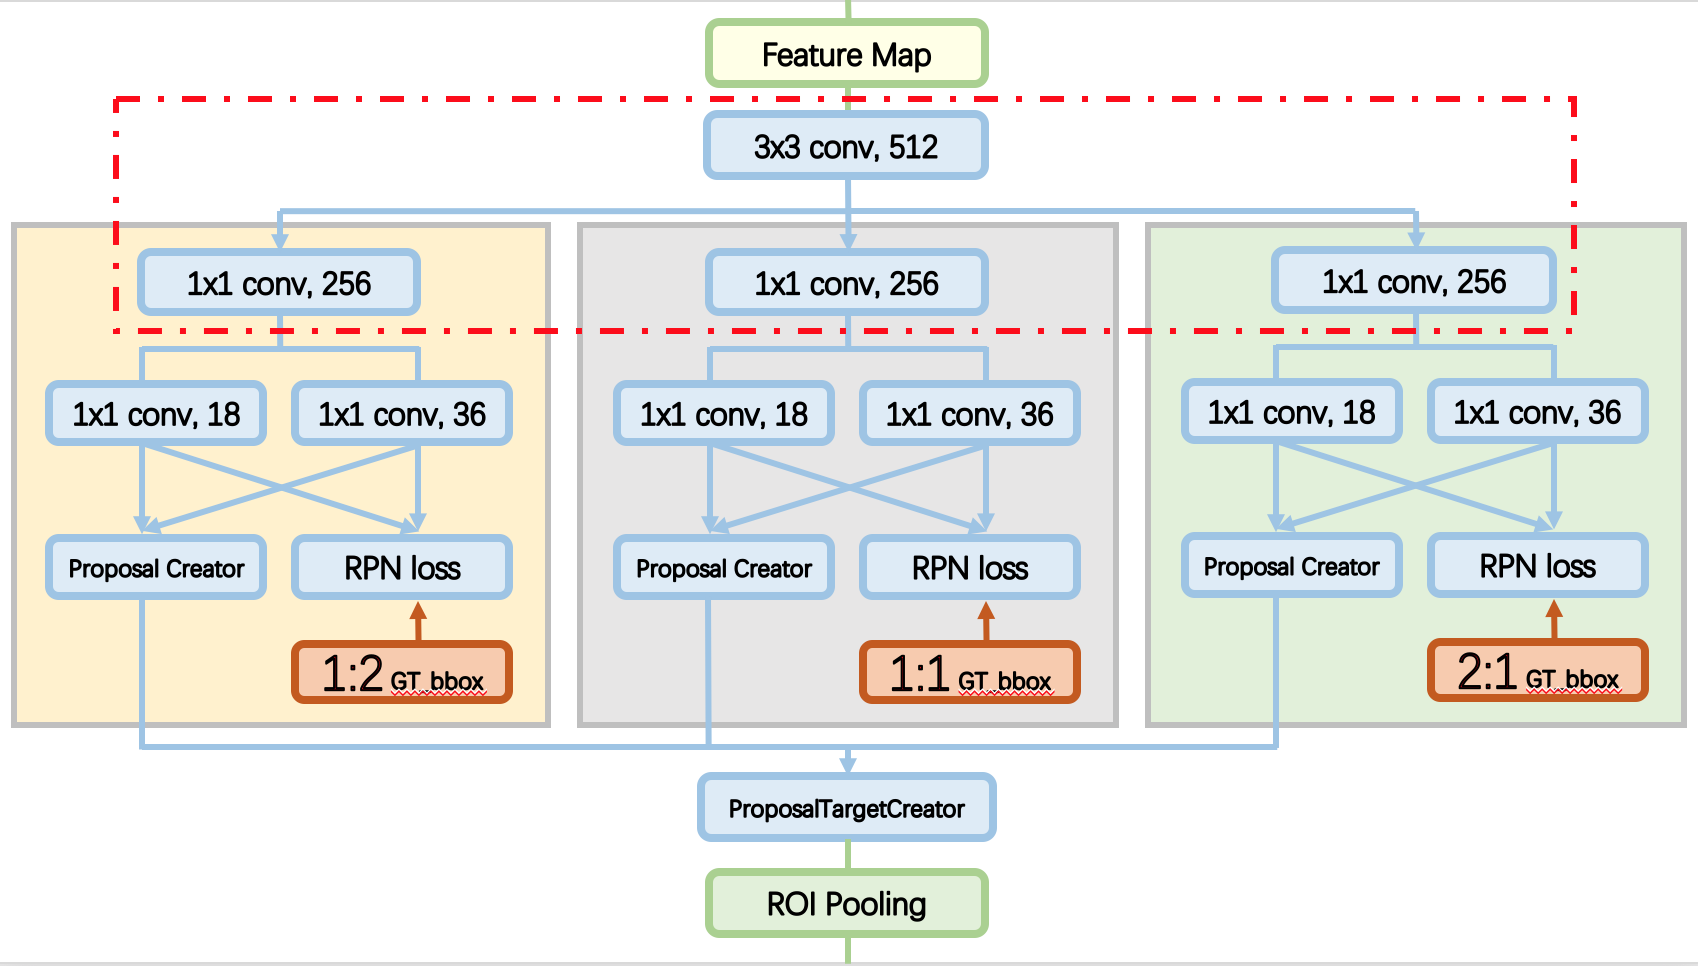
\includegraphics[width= 0.5\textwidth]{pic/ARS-archi-share.png}
    \caption{Sharing Features}
    \label{ARS_sh}
    \end{figure}

\begin{table}
\centering
\begin{tabular}{|c|c|}
\hline Approach & Frame per second (fps) \\
\hline ARSnet (300 proposals) & 4.73 \\
\hline ARSnet (900 proposals) & 3.56 \\
\hline ARSnet+1*1 conv (300 proposals) & 5.04 \\
\hline ARSnet+1*1 conv (900 proposals) & 3.84 \\
\hline faster RCNN (300 proposals) & 9 \\
\hline
\end{tabular}
\caption{Time complexity under different settings reported on Nvidia TitanX. Adding 1*1 conv into our network improves speed while maintaining a similar mAp.}
\label{table_fps}
\end{table}

\subsection{Training Details}
In general, we adopted the training approaches from the origin faster RCNN. Fisrt 30 feature extraction layers are initialized with a pretrained VGG-16 model from caffe, other convolutional layers are drawed from a zero-mean Gaussian distribution with standard deviation with 0.01 (\emph{REF FAST RCNN}). One single image is chosen randomly at each step to provide positive and negative samples up to 1:3 ratio for both rpns and final classifiers. We trained the network with stochastic gradient descent (SGD) end-to-end, learning rate is set to 0.001 for the first 15 epochs. Then we fine-tuned the model with the best accuracy with another learning rate of 0.0001 for the next 15 epochs. Our approach shows an significant increase of aspect ratio sensitive class.



\section{Experiment}
\subsection{Experiments on PASCAL VOC}
We evaluate our method on the PASCAL VOC 2007 detection benchmark. This dataset consists of 5011 train images and 4952 test images over 20 object categories. Evaluation is perforated on all test images. The metric we use is mean Average Precision (mAP). This is also a general metric in the field of computer vision.
(How about recall)\\
\indent{}We applied our method to Faster R-CNN with the public VGG-16 model, which has 13 convolutional layers and 3 fully-connected layers. Table 1 shows the results on VGG-16 model. Using ARS Net, the result is 73.2\% for shared features between proposal and detection, compared to 71.8\% that evaluated on single RPN. As shown above, our method has also dramatically improved AP in some categories such as bottle (by 3.9\%) and cow (by 5.9\%). This is because we specify each RPN processing selected ground truth during training, which leads to the aspect ratio sensitivity. Thus the proposals generated by ARS Net for those categories are more accurate. There's a slight decrease in several classes, which is a side effect. One possible reason is that the distribution of the test set is not consistent with the training set.

\subsection{Number of Proposals}
We further tested ARS Net with diverse number of proposals, which is as shown in Table 2. When the number of proposals drops from 900( Top 300 proposals are selected from each scale) to 300, mAP reduce by X\%. And a further decrease on proposals leads to dropping on mAP. (What?s the reason).
In fact, when number of proposals is 400 each, mAP reaches the highest. However, this will lead to a decrease in fps.




% speed
% overall performance

\section{Discussion}
% other ways to split the dataset?

{\small
\bibliographystyle{ieee}
\bibliography{egbib}
}

\end{document}
